\documentclass[11pt,a4paper]{article}

\usepackage[T1]{fontenc}
\usepackage[utf8]{inputenc}
\usepackage{lmodern}
\usepackage[margin=2.3cm]{geometry}
\usepackage{amsmath}
\usepackage{booktabs}
\usepackage{graphicx}
\usepackage{xcolor}
\usepackage{microtype}
\usepackage[colorlinks=true,linkcolor=black,urlcolor=blue!60!black]{hyperref}
\usepackage{caption}
\captionsetup{font=small,labelfont=bf}

\setlength{\parskip}{0.42em}
\setlength{\parindent}{0pt}

\title{\vspace{-1.7cm}\large Divergence-form and wide-halo mEVP in the GPU version of FESOM2:\\
what was built, and what it costs}
\author{\normalsize Nikolay Koldunov}
\date{\normalsize 6 August 2026}

\begin{document}
\maketitle
\vspace{-1.1cm}

\section*{1. What this note is about}

Two of your proposals were implemented in our GPU version of FESOM2 and measured:
\textbf{(a)} the \textbf{reformulation of the mEVP sub-cycling} in which the quantity carried
from one sub-cycle to the next is the divergence of the stress, held at nodes, instead of the
three stress components held at elements; and \textbf{(b)} the \textbf{wide halo}, in which the
halo is exchanged only every $K$-th sub-cycle and the missing information is recomputed locally
in a ring of ghost cells $K$ deep, so that the result is identical to exchanging after every
sub-cycle.

A third option came out of the measurements and had to be included: simply exchanging every
$K$-th sub-cycle and letting the halo go stale. It is not exact, but it is by far the cheapest,
so its accuracy had to be established rather than assumed.

Everything below is measured on production configurations. Where something is not measured, that
is said.

\textbf{Two things are worth knowing before the detail.} First, we report every speed number in two
currencies --- percent of the whole model step and percent of the ice cost --- because the first
divides an ice-only change by ten and made us report your reformulation as a null result when it is
not (section~6.2). Second, the cheap option, the one that gives up exactness, turns out to \textbf{draw the domain
decomposition into the ice field} (section~6.6). It is the fastest thing we measured and it is not
usable; we report it as a measured negative.

\section*{2. Terms, configurations, meshes, machine}

\textbf{The sub-cycle and the halo.} mEVP advances the ice momentum with 120 sub-cycles per model
time step in all our configurations. The mesh is divided among MPI processes; each process owns a
piece of it and keeps a one-cell-wide copy (the \emph{halo}) of its neighbours' edge values. In
the standard scheme the ice-velocity halo is exchanged after \emph{every} sub-cycle, so one model
step costs 120 halo exchanges.

\textbf{The five configurations.} These names are used throughout.

\begin{center}\small
\begin{tabular}{@{}lll@{}}
\toprule
\textbf{name} & \textbf{carried between sub-cycles} & \textbf{halo exchange} \\
\midrule
standard & stress $\sigma_{11},\sigma_{12},\sigma_{22}$ at elements & after every sub-cycle \\
divergence form & $\nabla\!\cdot\!\sigma$ (two components) at nodes & after every sub-cycle \\
wide halo, standard form & stress at elements, ring $K$ deep & every $K$-th sub-cycle, \emph{exact} \\
wide halo, divergence form & $\nabla\!\cdot\!\sigma$ at nodes, ring $K$ deep & every $K$-th sub-cycle, \emph{exact} \\
delayed exchange & stress at elements & every $K$-th sub-cycle, \emph{stale halo} \\
\bottomrule
\end{tabular}
\end{center}

The two wide-halo configurations are exact in the strict sense: they reproduce the
every-sub-cycle trajectory bit for bit. The delayed exchange does not, and section~6.5 says by
how much.

\textbf{Meshes and machine.} All four are production configurations. Levante at DKRZ: GPU nodes
carry four NVIDIA A100 (80\,GB) and one MPI process per GPU; CPU nodes carry two AMD EPYC 7763,
128 cores each. Every comparison is made inside one job allocation with the same executable, and
is the faster of two repetitions; repetition spread is below 0.4\% on GPU and about 1.5\% on CPU.

\begin{center}\small
\begin{tabular}{@{}lrrrl@{}}
\toprule
& \textbf{surface nodes} & \textbf{elements} & \textbf{levels} & \textbf{time step} \\
\midrule
CORE2 & 126\,858 & 251\,746 & 48 & 1800\,s \\
fArc  & 638\,387 & 1\,270\,173 & 48 & 900\,s \\
DARS  & 3\,160\,340 & 6\,294\,801 & 57 & 120\,s \\
NG5   & 7\,402\,886 & 14\,827\,217 & 70 & 180\,s \\
\bottomrule
\end{tabular}
\end{center}

\section*{3. The problem}

One model step of the standard scheme performs 120 ice-velocity halo exchanges, each moving very
little data, with very little arithmetic between them. Koldunov et al.\ (2019, GMD 12, 3991)
diagnosed this on the fArc mesh and proposed --- without testing it --- ``wider halo regions to
reduce communication frequency''. The wide halo above is that proposal.

We can now put numbers on the diagnosis in our own code.

\textbf{On CPU}, at 2304 cores on fArc, the ice part is 13.2\% of the model step, and inside the
ice dynamics the time spent \emph{waiting} for MPI is 4.8\,ms per step against 3.5\,ms of actual
computation. The cost is idle time, not arithmetic.

\textbf{On GPU} the same structure costs more, for a second reason. Each exchange is a sequence of
small GPU operations --- gather the values to be sent, copy, scatter the values received --- and
each carries a fixed issue cost independent of how little data it touches. On CORE2 with 8 GPUs
the ice-dynamics phase takes 8.2\,ms per model step, of which only about 1.25\,ms is arithmetic,
spread over roughly 480 separate GPU operations.

\textbf{So the mEVP sub-cycle, as it stands, is limited by communication and by the number of
operations issued --- not by arithmetic and not by memory traffic.} This one fact explains every
result below, including the negative ones.

\section*{4. The code before this work}

FESOM2 (ocean and ice) has been rewritten in C++ with Kokkos and runs entirely on the GPU, with
no per-step transfer of prognostic fields to the host. On CPU it is bit-for-bit identical to our
validated C port of FESOM2, which was itself validated against Fortran FESOM2; on GPU it differs
only at the level of summation order, checked against the CPU version over multi-decadal
integrations. mEVP was already ported and validated, exchanging after every sub-cycle and keeping
the stress at elements --- that is, it was the ``standard'' row above, and it is the reference for
everything that follows.

\section*{5. What was implemented}

All four new configurations are selected at run time and are off by default, so the validated
path is untouched when they are not requested.

\textbf{The divergence form.} The stress recursion is replaced by a recursion for
$R=\nabla\!\cdot\!\sigma$ at nodes, with the ice-element mask applied so that $R$ is advanced
only where ice elements contribute.

\textbf{The wide halo, both forms.} At the start of each model step one extended exchange fills a
ring of ghost nodes and ghost elements $K$ cells deep with the owner's values of the eleven
fields the sub-cycle needs. Over the next $K-1$ sub-cycles each process advances that ring itself,
in the owner's order, and needs no communication; on the $K$-th sub-cycle the ring is refreshed.
The ring's geometry, boundary mask and per-step element quantities are shipped from their owners
rather than recomputed --- a locally recomputed value can differ in the last bit, and that is
enough to destroy exactness.

\textbf{The delayed exchange.} One conditional: the exchange fires only when the sub-cycle index
is a multiple of $K$. Nothing else changes.

\textbf{How correctness was established.} For the exact options the requirement is strict: with
the option on, the model must produce \emph{bit-for-bit} the same output as with it off. That was
verified for the wide halo in both forms at $K=4$ and $K=8$, and separately for the same machinery
under standard EVP. The options were also shown to leave the model unchanged when a different
vertical mixing scheme or vertical coordinate is selected, and the GPU version was checked against
the CPU version with the options on. The delayed exchange is an approximation, so bit-for-bit
equality is not available and its accuracy was measured instead (section~6.5).

\section*{6. Results}

\subsection*{6.1 The reformulation is exact in the discretisation}

Carrying $R$ and $\sigma$ simultaneously and comparing them sub-cycle by sub-cycle, $R$ agrees
with $\nabla\!\cdot\!\sigma$ to $1$--$2.5\times10^{-15}$ relative, and this does not grow over
20 model steps, i.e.\ 2400 sub-cycles. The algebra survives the discretisation to round-off, not
merely to plotting accuracy.

One genuine non-equivalence is worth naming. Within a model step the ice-element mask is fixed and
the two forms are equivalent. \emph{Across} steps, when an element enters or leaves the ice mask,
they are not exactly equivalent, because in the divergence form the recursion has already been
applied after summation over the elements around a node rather than before. We measured it: it
fires only on steps where mask membership actually changes, and is bounded by
$2.1\times10^{-11}$ relative. That is far below physical significance, but it means the divergence
form is not bitwise reproducible against the standard form over a long integration, and should be
introduced as a scheme change rather than as an optimisation.

\subsection*{6.2 The reformulation alone does not save time}

\textbf{First, the denominator, because it decides how this reads.} Percent of the \emph{model
step} is what a production run feels, but the ice is only a small part of a step --- 5 to 13\% on
CPU --- so an ice-only change is divided by 10 before it reaches that number. Percent of the
\emph{ice cost} (ice + ice dynamics + ice advection, computation \emph{and} MPI wait, which is the
definition Koldunov et al.\ 2019 used) is what judges a sea-ice scheme. We report both from here
on; quoting only the first is what made our first reading of this result wrong.

Measured against the ice cost, the reformulation \textbf{does} pay on CPU, and the more so the more
processes are used: $-2.2\%$ at 512 processes on fArc, $-3.2\%$ at 1024, $-5.6\%$ at 1536,
$-6.7\%$ at 2048, and $-8.5\%$ on CORE2 at 512. Against the model step the same runs read
$-0.5\%$ to $0\%$ --- which is why we first reported it as nothing.

On GPU it is a \emph{cost} in both currencies: $+2$ to $+17\%$ of the ice cost, $0$ to $+1.6\%$ of
the model step (the ice-dynamics phase alone grows 13\% on CORE2 with 8 GPUs, 7\% on NG5).

The reason is section~3. To bound the largest saving the reformulation could possibly deliver we
ran a control: three element-sized arrays that the mEVP path writes every sub-cycle and never
reads were simply not written. That removes strictly more memory traffic than the reformulation
does, and it changed the run time by \textbf{exactly 0.00\%}. There was no memory-traffic saving
available to collect. Profiling agrees from the other side: total GPU arithmetic time is identical
in the two forms, 21.8 against 21.7\,ms per step.

So the honest verdict is \textbf{backend-split, not null}: the reformulation removes real work,
but on GPU it removes work that was not being paid for, because there the sub-cycle is limited by
the number of operations issued rather than by arithmetic or memory traffic. On CPU, where that is
not the case, it is worth having.

\textbf{One caveat} we would rather state than hide: the CPU numbers at the largest process counts are
wait-dominated and noisy --- at fArc with 2048 processes the ice cost falls 6.7\% while the model
step \emph{rises} 1.0\%, which is not internally consistent and is probably load-imbalance jitter.
The CORE2 512-process point ($-8.5\%$ of the ice, $-0.34\%$ of the step, same sign) is the cleaner
one. These deserve a re-measurement on matched instrumented pairs before they are quoted in a
paper.

\begin{figure}[tb]
\centering
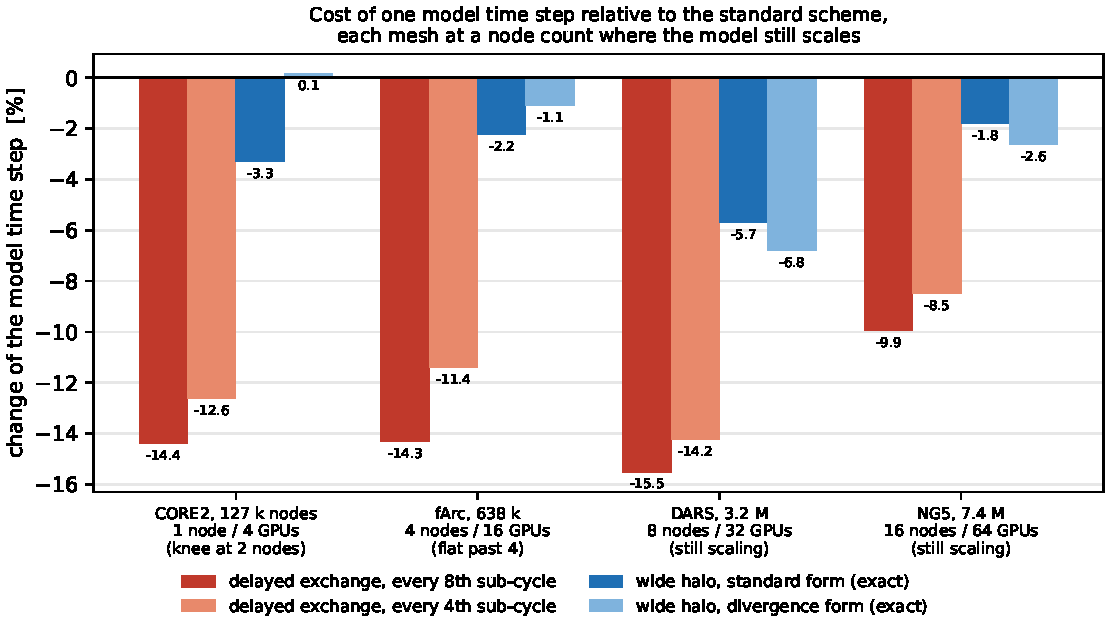
\includegraphics[width=\textwidth]{fig1_meshes.pdf}
\caption{Cost of one model time step relative to the standard scheme (exchange after every
sub-cycle). Negative is faster. \textbf{Each mesh is shown at its own operating point} --- the
largest node count at which the model still gains from more GPUs, read off the measured
strong-scaling curve --- rather than at a common node count, which would have flattered every
option: CORE2 on 16 nodes gives $-25.5\%$ for the delayed exchange and is 45\% slower there than
on two nodes. Each mesh was measured in a single allocation with all configurations run back to
back. The two wide-halo bars are \emph{exact} --- they reproduce the standard trajectory bit for
bit --- while the two delayed bars are approximations whose accuracy is
Figure~\ref{fig:accuracy}.}
\label{fig:meshes}
\end{figure}

\subsection*{6.3 The wide halo works, and is worth a few percent on GPU}

Figure~\ref{fig:meshes} is the summary of the speed results. Every mesh there is shown at
\emph{its own operating point} --- the largest node count at which the model still gains from
more GPUs, read off the measured strong-scaling curve. That matters: at a common large node count
these numbers roughly double, but a configuration past its scaling limit is not one anybody runs,
and quoting it would flatter every option in this study.

Reading the figure:

\begin{itemize}\itemsep0.12em
\item The wide halo is a real gain and it is \emph{exact} --- there is no accuracy argument to
make --- worth $-1.8$ to $-6.8\%$ of the model step at realistic operating points, which is
\textbf{$-12$ to $-19\%$ of the ice cost} (fArc, 16 GPU nodes, $K$=8: $-11.9\%$ in the classic
form, $-19.1\%$ in the divergence form). \textbf{That $-19.1\%$ is the same configuration and the
same number as your own $\sim$20\%} --- there was never a disagreement, only a denominator.
\item It is worth substantially less than the delayed exchange on every mesh.
\item On CPU it never wins, on any mesh, at any $K$.
\item It needs large $K$. At $K=2$ it is a net \emph{cost} on most configurations, because the
duplicated ring has not been amortised. This is the opposite of what the delayed exchange wants
(section~6.5), so the two options do not share a best $K$.
\end{itemize}

\textbf{This reproduces, and sharpens, an earlier assessment.} Our optimisation campaign measured
the wide halo under standard EVP a month ago --- NG5, 4 and 16 GPU nodes --- and got
$+1.7\%$ at $K=4$ and $-2.2\%$ at $K=8$, i.e.\ ``low yield''. Re-measured this week at the same
point with the current code: $+1.69\%$ and $-2.26\%$. The earlier number was right. What that
campaign also noted at the time, and never acted on, was that its wide refresh sent
\emph{two messages per neighbour} and that fusing them into one was a candidate fix; doing that
now takes NG5 from $-2.26\%$ to $-4.19\%$ at $K=8$ and from $+1.69\%$ to $-2.47\%$ at $K=4$. So
the fusion is worth roughly 2 to 4 percentage points --- real, and not enough to change the
verdict on NG5.

The CPU result has a clear mechanism, and it is the most useful thing the wide halo taught us.
Trading communication for local recomputation is profitable only while the ring stays small
relative to the sub-domain \emph{and} a message stays expensive relative to the recomputation. The
controlling quantity is the ratio of ghost cells that must be advanced to owned cells, which grows
like $K\times(\text{perimeter}/\text{area})$ of the sub-domain. On GPU, where a process holds a
large piece of the mesh, that ratio is 0.03 to 0.25 and the wide halo pays. On CPU, where
processes are small and messages are comparatively cheap, it is 0.19 to 1.18 and it never did: on
fArc with 2048 processes at $K=4$ the ratio reaches 1.18 --- the ring a process must advance is
\emph{larger than its own sub-domain} --- and that configuration costs 5 to 7\% instead of saving
anything.

A second effect pushes the same way. The ring is a different size on every process, so duplicating
it introduces a new load imbalance on top of the one it removes: on fArc CPU the ice-dynamics
waiting time rose from 8.7 to 25.3\,ms per step when the ring was made deep.

\subsection*{6.4 The delayed exchange is the largest gain}

Accepting a halo up to $K-1$ sub-cycles old removes 105 of the 120 exchanges per step at $K=8$ and
costs one conditional. At the four operating points of Figure~\ref{fig:meshes} it is worth
$-14.4$, $-14.3$, $-15.5$ and $-9.9\%$ of the whole model step at $K=8$ (CORE2, fArc, DARS, NG5),
and $-12.6$, $-11.4$, $-14.2$ and $-8.5\%$ at $K=4$. On CPU the same change is worth $-1$ to
$-3.4\%$, because a CPU process holds far less of the mesh and the ice exchange is a much smaller
share of its step. For scale, the largest single code optimisation this port had previously
achieved was about 8\%.

Against the ice cost the same option is worth \textbf{$-37$ to $-58\%$ on GPU} and $-5$ to $-25\%$
on CPU (growing with process count: $-5\%$ at 128, $-25\%$ at 2048).
\textbf{$K=4$ retains about 90\% of the gain of $K=8$}, which matters because the accuracy evidence
pushes the other way.

\begin{figure}[tb]
\centering
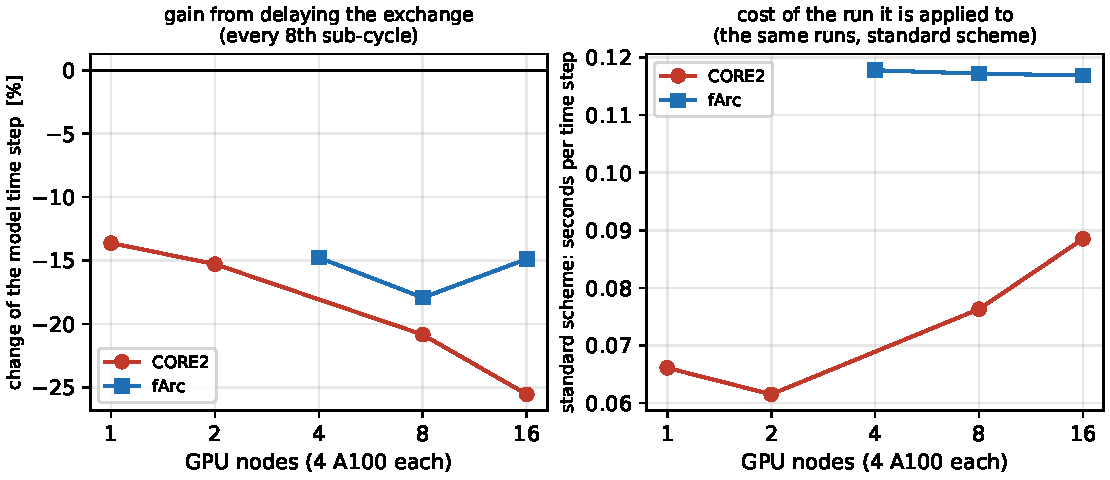
\includegraphics[width=\textwidth]{fig2_scaling.pdf}
\caption{Why the gain from delaying the exchange varies. \emph{Left}: change of the model time
step from exchanging every 8th sub-cycle instead of every one. \emph{Right}: the cost of the very
same runs under the standard scheme. The gain is largest where the model has stopped scaling and
communication dominates --- CORE2 past two nodes, where adding GPUs makes the model \emph{slower},
is exactly where the delayed exchange recovers the most.}
\label{fig:scaling}
\end{figure}

Figure~\ref{fig:scaling} shows why the gain varies, and it is a caution as much as an
explanation. It is not simply larger with more processes: it tracks how much communication the run
is already paying for. CORE2 on GPU stops scaling at two nodes and then \emph{degrades} --- more
GPUs, slower model --- and that is exactly where the delayed exchange recovers the most, $-25.5\%$
at 16 nodes. That number is real but useless: it is measured in a configuration one would never
run, and it is why Figure~\ref{fig:meshes} quotes operating points instead. The same variable
works in the other direction too --- on NG5 spread over only four nodes, 460\,000 mesh nodes per
GPU, nothing we tried moved the model by more than 3\%.

The mechanism was measured directly, and it is the one the 2019 paper describes: on fArc with 2304
CPU cores the ice-dynamics waiting time falls from 4.8 to 1.9\,ms per step (a 60\% cut) while the
computing time barely moves, and MPI operations per step fall from 240 to 30. \textbf{The gain
comes from removing idle time, not from computing faster.}

\subsection*{6.5 What the delayed exchange costs in accuracy}

This decides whether the option is usable, so the test was specified in advance and then measured:
one-year CORE2 integrations at $K=2,4,8$ against the same run exchanging after every sub-cycle, on
the CPU backend, which is exactly reproducible --- so every difference seen is the approximation
and nothing else. (On GPU, run-to-run differences in summation order accumulated over a year are
the same size as the effect being measured, so the GPU cannot answer this question; we confirmed
it agrees to that resolution.)

The yardstick is mEVP's own reproducibility: the difference between two independent, both correct,
implementations of the same scheme --- our C port and Fortran FESOM2 --- over the same year.

\begin{center}\small
\begin{tabular}{@{}lcccccc@{}}
\toprule
pattern correlation after 1 year & SST & SSH & ice conc. & ice thickness & $u_{\rm ice}$ & $v_{\rm ice}$ \\
\midrule
C port versus Fortran (the yardstick) & 1.00000 & 1.00000 & 0.99999 & 0.99998 & 0.95438 & 0.93908 \\
delayed exchange, $K=2$ & 1.000000 & 1.000000 & 0.999996 & 0.999998 & 0.970111 & 0.952946 \\
delayed exchange, $K=4$ & 1.000000 & 1.000000 & 0.999995 & 0.999994 & 0.963328 & 0.950003 \\
delayed exchange, $K=8$ & 1.000000 & 1.000000 & 0.999992 & 0.999981 & 0.961359 & 0.944857 \\
\bottomrule
\end{tabular}
\end{center}

Every field stays inside the yardstick at every $K\le8$ (Figure~\ref{fig:accuracy}). But the margin
should be read, not just the verdict: on ice velocity the approximation sits only 1.1 to 1.5 times
inside it, and at $K=8$ ice thickness is only 1.05 times inside. We had expected an order of
magnitude and were wrong. The delayed halo's effect on the velocity field is of the same order as
the spread between two implementations of mEVP --- comfortably inside it at $K\le8$, but not by
much.

Two further results:

\begin{itemize}\itemsep0.12em
\item The error is \textbf{monotone in $K$} when measured as RMS difference or correlation. (It is
not monotone in the maximum pointwise difference, which is carried by one to five points at the ice
edge and is not a usable statistic here.)
\item \textbf{Integrated ice quantities are untouched.} The largest monthly deviation in Northern
Hemisphere sea-ice extent at $K=8$ is $0.022\times10^{6}$\,km$^2$ against a seasonal range of
$7.8$ to $17.5\times10^{6}$\,km$^2$ --- 0.23\% of the amplitude. Surface temperature, salinity and
sea surface height correlate at 1.000000 at every $K$: over a year the change does not reach the
ocean surface climate.
\end{itemize}

On this evidence we would use $K=4$: it keeps most of the speed, and since the error is monotone in
$K$, the smallest $K$ that pays is the defensible choice. \emph{This is measured at CORE2
resolution only}; see section~8.

\begin{figure}[tb]
\centering
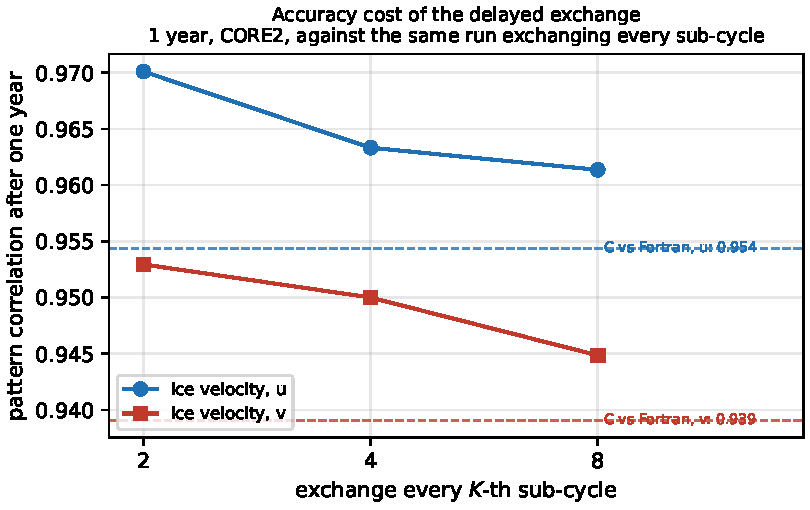
\includegraphics[width=0.70\textwidth]{fig3_accuracy.pdf}
\caption{Accuracy cost of the delayed exchange on the field that carries it. One-year CORE2
integrations on the CPU backend (exactly reproducible, so the whole difference is the
approximation), against the same run exchanging after every sub-cycle. Dashed lines: the same
correlation between two independent and both-correct implementations of mEVP --- our C port and
Fortran FESOM2 --- over the same year. The approximation stays inside that spread at every $K$
tested, by a factor of 1.1 to 1.5.}
\label{fig:accuracy}
\end{figure}

\subsection*{6.6 The delayed exchange draws the decomposition into the ice --- and that rules it out}

This was raised as an objection --- would the stale halo show up as partition artefacts in the ice?
--- and it turned out to be the finding that decides the recommendation.

The concern is well posed. The stale values sit on exactly the one-cell rim of each sub-domain,
and the partition is fixed for the whole run, so the same nodes are perturbed at every step of
every day. A global correlation cannot see it: a one-cell-wide feature along sub-domain edges is a
small fraction of the mesh and can leave a domain-wide correlation at 0.99999 while being obvious
on a map.

\textbf{Test.} fArc, 16 GPUs, 60 days with daily ice output, all configurations from the same
binary and the same 16-way partition. For each node we take its distance in elements from a
sub-domain boundary and average $|\Delta$ ice thickness$|$ over the 60 days within each ring. If
the option imprints the decomposition the average must peak at the boundary and decay; if it does
not, the profile is flat. \textbf{Two negative controls make the test falsifiable}: two identical
runs (whose only difference is the order of summation on the GPU), and the exact wide halo (which
is bit-identical in exact arithmetic, so it should behave like the control).

\begin{center}\small
\begin{tabular}{@{}lrrr@{}}
\toprule
& rim & interior & \textbf{edge/interior} \\
\midrule
two identical runs --- control & 0.00105\,m & 0.00124\,m & \textbf{0.85} \\
\textbf{wide halo, exact, $K$=8} & 0.00104 & 0.00120 & \textbf{0.87} \\
delayed exchange, $K$=2 & 0.00432 & 0.00249 & \textbf{1.70} \\
delayed exchange, $K$=4 & 0.01178 & 0.00452 & \textbf{2.52} \\
\bottomrule
\end{tabular}
\end{center}

\textbf{The delayed exchange imprints the partition; the exact wide halo does not.} The two
controls land together at 0.85 and 0.87, which is what validates the diagnostic --- an exact
option is measured as having no imprint, by the same statistic that finds one in the
approximation. The effect is present on \textbf{day one} (ratio 3.1, when the difference is still
$10^{-4}$\,m), persists for two months, scales with $K$, and appears in ice concentration (2.86)
and ice velocity (1.76) as well as thickness. Figure~\ref{fig:artefact} shows both the ring
profiles and the map: the difference field traces the sub-domain boundaries.

\textbf{Why this rules the option out, and it is not the accuracy cost.} Section~6.5 remains
true: the delayed exchange stays inside mEVP's own implementation spread, and every integral
diagnostic is untouched. The objection is different in kind. The error is not distributed like an
implementation difference --- it is a \emph{polygonal structure in a physical field, in the shape
of the processor grid}. A sea-ice field with the decomposition visible in it is not something one
can put in front of a sea-ice modeller, whatever the correlation coefficient says, and no amount
of speed buys that back. (That the pattern also changes with the core count is true but secondary;
these models are not bit-reproducible across decompositions anyway, and nobody objects to that.)
Reducing the delay to $K$=2 halves the ratio, to 1.70, but does not remove it.

\textbf{It also draws the line your own message drew, and confirms it.} Giving up bit-identity by
\emph{recomputing} a shared quantity independently --- each core changing the last bit on a
triangle it shares --- is harmless: that is precisely our control, and it measures 0.85. Giving it
up by \emph{reading a halo that is $K-1$ sub-cycles old} is not the same thing at all: that is a
physical-magnitude error injected at the rim, and it measures 2.52. The wide halo recomputes; the
delayed exchange stales. Only the second imprints.

\begin{figure}[tb]
\centering
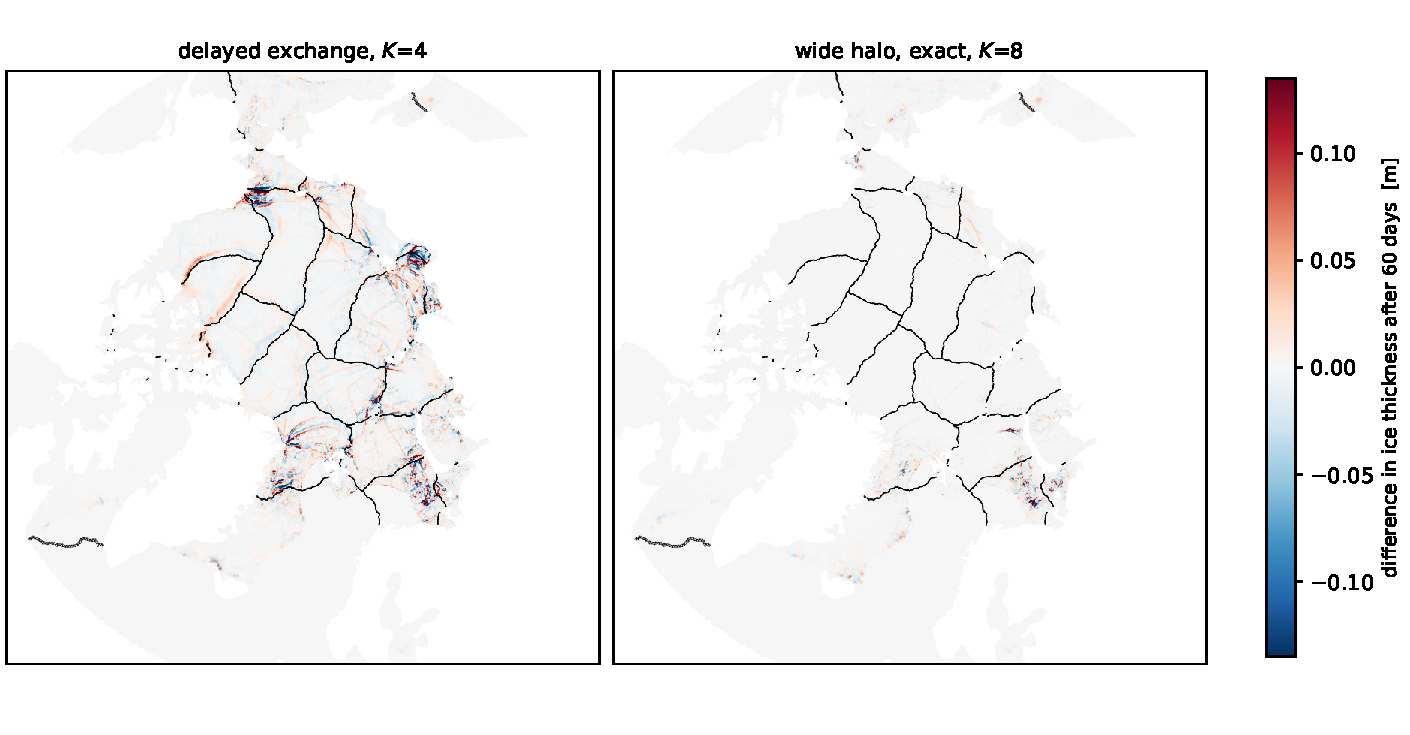
\includegraphics[width=\textwidth]{fig4_artefact.pdf}
\caption{\emph{Left}: mean $|\Delta$ ice thickness$|$ over 60 days against distance from a
sub-domain boundary, fArc on 16 GPUs; open markers are the interior. The two exact configurations
(control, wide halo) are flat; the two approximate ones peak at the boundary and decay. Bracketed
numbers are the edge/interior ratio --- 1 means no imprint. \emph{Right}: the day-60 difference
for the delayed exchange at $K$=4 with the 16 sub-domain boundaries drawn on top.}
\label{fig:artefact}
\end{figure}

\subsection*{6.7 Why the divergence form's expected advantage did not survive}

This is the result we would most like your view on, because it corrects something we believed
until two days ago.

The two wide-halo forms differ in what they must send. The standard form must send node velocities
\emph{and} the ghost ring's element stresses --- in our implementation, two messages per
neighbour. The divergence form sends one message, because everything it carries lives at nodes,
and it sends about half as many numbers. We measured the divergence form to be the faster of the
two on every GPU mesh, by up to 7 percentage points of the model step, and attributed that to the
smaller volume --- which is the advantage the reformulation is designed to deliver.

That attribution was wrong. We changed the standard form to pack its two pieces into a
\emph{single} message per neighbour --- identical values in identical order, verified bit for bit
against the two-message version --- and the difference reversed. Holding the volume fixed and
removing one message is worth up to 8.6 percentage points of the model step; holding the message
count fixed and removing 19\% of the data is worth nothing. On DARS with 32 GPUs the two
configurations then send \emph{exactly} the same number of messages (24\,400 per step) while the
divergence form sends 19\% fewer numbers --- and the divergence form is 1.3 percentage points
\emph{slower}, because it must reconstruct the ghost ring's stresses in an extra pass.

Across ten configurations where all three variants ran side by side, removing the message helps
everywhere ($-0.1$ to $-8.6$ percentage points), while halving the data is worth between $-1.3$ and
$+2.8$ points and favours the \emph{standard} form in eight of the ten.

The conclusion is not that the reformulation is wrong --- section~6.1 shows it is exact --- but
that on this hardware the cost of an exchange is dominated by the per-message overhead rather than
by its volume, so halving the volume buys nothing that the extra local pass does not immediately
give back. Across fourteen configurations the two forms now sit within about 1.5 percentage points
of each other, with the standard form ahead in ten of them; where the divergence form wins --- DARS
and NG5 --- it wins by about one point. Neither is systematically better.

\section*{7. Where this leaves the three ideas}

\begin{center}\small
\begin{tabular}{@{}p{3.0cm}p{5.2cm}p{7.3cm}@{}}
\toprule
& \textbf{status} & \textbf{our reading} \\
\midrule
divergence form &
exact to round-off; on CPU $-2$ to $-8.5\%$ of the ice cost, growing with process count; on GPU a
cost of $+2$ to $+17\%$ &
\textbf{not a null result} --- our first report of it as one came from quoting percent of the model
step, where the ice is a tenth of the total. It removes real work; on GPU that work was not being
paid for, because the sub-cycle there is limited by operation count. \\[0.3em]
wide halo (either form) &
exact, bit for bit; $-12$ to $-19\%$ of the ice cost on GPU at $K$=8 ($-2$ to $-7\%$ of the model
step); never profitable on CPU; \textbf{no partition imprint} &
\textbf{the option we would put into production.} It is the only one that is both worth having and
free of an accuracy argument and of an artefact. Its $-19.1\%$ of the ice cost on fArc is the same
measurement as your $\sim$20\%. \\[0.3em]
delayed exchange &
approximate; $-37$ to $-58\%$ of the ice cost on GPU --- three times the wide halo --- but
\textbf{it draws the sub-domain boundaries into the ice} (edge/interior 2.52 at $K$=4 against a
control of 0.85, and still 1.70 at $K$=2) &
\textbf{a no-go, and reported as a measured negative.} It is the fastest thing in this study and
it cannot be used: a polygonal artefact in the shape of the processor grid disqualifies a sea-ice
scheme regardless of how small the integral error is. Worth knowing about, and worth the
measurement, but not an option. \\
\bottomrule
\end{tabular}
\end{center}

\section*{8. What has not been measured}

\begin{itemize}\itemsep0.12em
\item \textbf{The accuracy of the delayed exchange at high resolution} was going to be the
largest remaining gap. It is now moot: section~6.6 rules the option out on other grounds, so the
one-year CORE2 accuracy result stands as a record of what the approximation costs, not as support
for using it.
\item \textbf{A leaner wide halo.} Our implementation ships eleven auxiliary fields once per step
so that rings 2\dots$K$ --- which do not exist in FESOM's data structures --- have any values at
all. Measured, that ship is 1.6--6.2\% of the wide halo's messages and 3.6--9.2\% of its bytes, so
removing it entirely could buy at most a few tenths of a percent of the model step. Your scheme
avoids it by staying inside the halo FESOM already maintains, which is also why it is limited to
$K$=2. We have not implemented that variant.
\item \textbf{The divergence form over a long integration.} Since it showed no speed benefit we did
not carry it through a one-year test, so the $2.1\times10^{-11}$ per-step non-equivalence of
section~6.1 has not been followed to its long-term consequences.
\item \textbf{Core counts above 2304 on fArc.} The 2019 paper reaches 6912. The partition set we
have for that mesh stops at 2304, and the separately partitioned copy in the shared archive does
not run in this port (the ocean solver fails to converge immediately, at every time step tried,
which is a configuration problem rather than a stability one). Our measured ice share reaches 13\%
at 2304 cores where the paper interpolates 25--30\%; the two candidate reasons --- this port's own
communication optimisations, and mEVP here versus standard EVP there --- are untested.
\item \textbf{The 13\% GPU cost of the divergence form} (section~6.2) is measured but not
explained. It is not arithmetic time and not the masked node kernel; we have no mechanism for it
and are not offering one.
\end{itemize}

\vspace{0.5em}
{\footnotesize All configurations are switchable at run time in the port; the underlying runs, job
scripts and the full internal write-up can be shared on request.}

\end{document}
